\documentclass[10pt]{article}
\usepackage[top=1cm, bottom=1cm, left=1cm, right=1cm]{geometry}
\usepackage{graphicx}
\usepackage[colorlinks=true]{hyperref}
\usepackage{verbatim}
\usepackage{enumerate}

\title{Eclipse Wesnoth UMC Plugin Readme\\ Google Summer of Code 2010 Project}
\author{Timotei Dolean - \href{mailto:timotei21@gmail.com}{timotei21@gmail.com}}

\begin{document}

\maketitle

\tableofcontents
\setcounter{tocdepth}{3}
\newpage

\newcounter{cnt}
\newcommand{\icnt}{ \stepcounter{cnt} \thecnt }

\section{Foreword} \hskip\parindent
Through this readme the following terms with the specified meaning will be used:
\begin{enumerate}
\item Navigator - an Eclipse view that shows the projects in the workspace
\item Project - a directory on the harddrive that is represented as a top directory in the navigator.
\item Container - this is a directory or a project. Basically it can contain any file or directory children.
\end{enumerate}

The following image will highlight the terms used: 1 - Navigator, 2 - Project, 3 - Containers, 4 - Map files, 5 - Config files that contain WML code

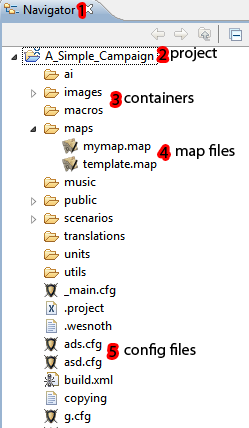
\includegraphics{definitions.png}

\section{Common prerequisites}
\begin{enumerate}
\item Download and install Sun's Java:
\begin{enumerate}
\item If you are going just to use the plugin (User): \href{https://cds.sun.com/is-bin/INTERSHOP.enfinity/WFS/CDS-CDS_Developer-Site/en_US/-/USD/ViewProductDetail-Start?ProductRef=jre-6u21-oth-JPR@CDS-CDS_Developer}{Download JRE}
\item If you are going to modify it or run it from source (Developer): \href{http://java.sun.com/javase/downloads/widget/jdk6.jsp}{Download JDK}
\end{enumerate}
\textit{Note:} Please double check the java installed on your system. On some machines there is the OpenJDK or other Java versions. Use just Sun's so there will be no problems.
\item Download ``Eclipse" (The download links are in the right. Please ensure you are downloading the \textbf{3.6} version, otherwise the plugin will not work.):
\begin{enumerate}
\item If you are going just to use the plugin (User): \href{http://eclipse.org/downloads/packages/eclipse-classic-360/heliosr}{Download Eclipse Classic}
\item If you are going to modify it or run it from source (Developer):  \href{http://eclipse.org/downloads/packages/eclipse-rcp-and-rap-developers/heliosr}{Download Eclipse for RCP and RAP Developers}
\end{enumerate}
\item Extract the downloaded archive in a known location and launch the executable (eclipse / eclipse.exe)
\end{enumerate}

\section{User}
\subsection{Installing the plugin}
\begin{enumerate}
\item After launching Eclipse, go to the ``Help'' menu - Install new Software.\\
  Then, please check ``Group items by category" and ``Contact all update sites during install to find required software", in the bottom of the page.\\ 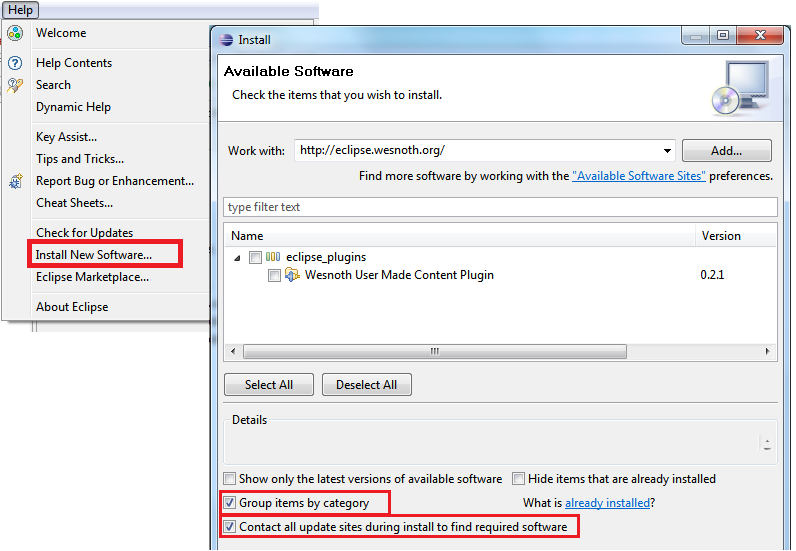
\includegraphics[width=550px]{install_new_software.png}
\item Insert the link \textbf{http://eclipse.wesnoth.org/} in the textbox in the top and press Enter. The list will be populated with some items.
\item Select the entire ``Wesnoth UMC Plugin" category and press finish.

\textit{Note:} If you are prompted for any license agreements or certificates press Yes on all (if you agree).\\
\textit{Note:} After the plugin has installed, press ``Restart workbench now" when you are prompted.
\item Now the plugin is ready to be used.
\end{enumerate}

\section{Developer}
\subsection{Setup the environment}
\begin{enumerate}
\item Checkout the following folders: ``org.wesnoth", ``org.wesnoth.wml'', ``org.wesnoth.wml.ui" from plugin's folder in the svn (http://svn.gna.org/svn/wesnoth/trunk/utils/java/)
\item In Eclipse, right click in \textbf{Package Explorer/Navigator/Project Explorer} and then select \textbf{Import - General - Existing projects into Workspace}
\item Select the path where you downloaded the java folder, and check all the 3 projects: ``eclipse\_plugin", ``org.wesnoth.wml'', ``org.wesnoth.wml.ui".
\item Build the projects.
\end{enumerate}

\subsection{Running the plugin} \hskip\parindent
After you've setup the environment and built the plugin you can run it.
\begin{enumerate}
\item Press the dropdown arrow near the ``Run" button in Eclipse's toolbar.
\item Press ``Run Configurations...".
\item Select ``Eclipse Application" from the category list in the left and then pres the left-most icon, to create a new run configuration.
\item Specify a name for the configuration
\item Press Run.
\end{enumerate}
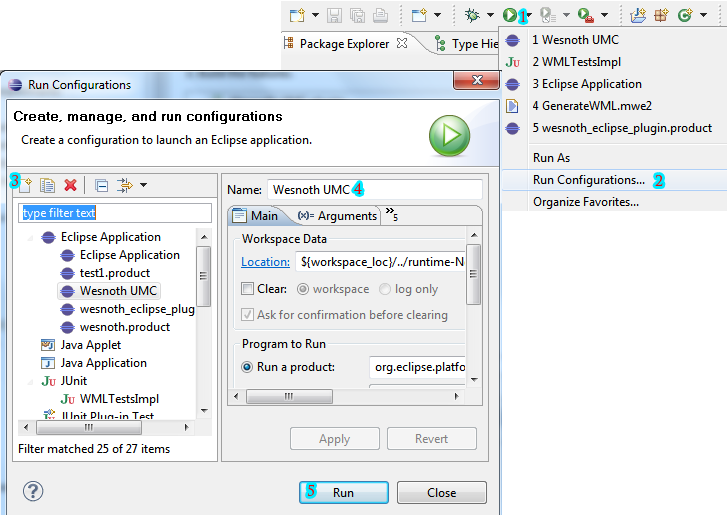
\includegraphics[width=550px]{launch_plugin.png}

\section{Everybody}
\subsection{Using the plugin} \hskip\parindent
After you have your plugin installed (user) or running(developer), you can use its features.

But before of all, you must ``Setup the workspace". For this, go in the ``Wesnoth" menu (it will have the wesnoth icon) and select ``Setup the workspace". You will be guided setting the workspace. The preferences page for the plugin will pop up, and you must fill them all, so the plugin will work as intended. After you completed the fields, press \textbf{Apply} and then \textbf{OK}. Then the plugin will create for convenience wesnoth projects for each of mainline campaigns and for each directory in your \textbf{useraddons/data/add-ons} directory. The working directory is the directory that contains the data, images, manual, sounds of wesnoth.

If there were no errors a message window will open saying: \textbf{Workspace was setup successfully}.

\textit{Note:} If you encounter any errors, the plugin logs them in the: \textbf{\textless your temporary directory\textgreater /wesnoth\_plugin/logs}.
That is usually on linux:\\
\indent \textbf{/tmp/wesnoth\_plugin/logs}\\
or on windows:\\
\indent \textbf{C:/Documents and settings/\textless your username\textgreater/Local Settings/Temp/wesnoth\_plugin/logs} \\
or\\
\indent \textbf{C:/Users/\textless your username\textgreater/Local Settings/Temp/wesnoth\_plugin/logs}

\subsubsection{Wizards} \hskip\parindent
There are some wizards available in the plugin, that will create either projects or config files, based on the specified input. This wizards are available by going to the ``File" menu - New - Other... , and from that list selecting the ``Wesnoth" category.

There are 3 wizards categories:
\begin{enumerate}
\item Project wizards - ``Empty project" and ``Campaign" wizards create new projects in the workspace. The former will create a basic addon directory structure. The latter will create a campaign and it's directory structure.
\item File wizards - ``Wesnoth config file", ``Scenario", ``Era" and ``Faction" wizards create a new file in a selected container.
\item Wizard launcher - This is a special wizard. It takes a wml tag as input, and generate subsequent needed tags and key inputs. This is generated on the wml schema, so if the schema is incomplete some tags won't be available. This wizard can create a new file or copy the resulted WML into the current edited file.
\end{enumerate}

\subsubsection{Menus} \hskip\parindent
There are currently 2 types of menus: the context menus for different file/container types and the main menu. For a better distinction the menus have the wenoth icon near each item.

\begin{description}
\item{\textbf{Project context menu}} - right click on the projects created with the plugin

   \textit{Wesnoth project report} - will show a simple report with the numer of maps, scenarios and units.\\
   \textit{Open campaign in game} - will start the current project's campaign (if any) in wesnoth. For this to work, you must have a ``\_main.cfg" file defined, and a campaign in it.\\
   \textit{Upload addon} - will upload the specified directory on the wesnoth addon server. The status will be outputed to the console.\\
   \textit{Regenerate build files} - recreates the ``build.xml" file. That is used if the current project is one relative to useraddons\\
   \textit{Builders} - utilities for adding/removing the wesnoth/xtext builders. Don't use them until you know what you are doing.

\item{\textbf{Container context menus}} - right click on any container

    \textit{WML Tools} - provides some options for using the wmltools with the specified project.

\item{\textbf{``maps" folder context menu}} - right click on the ``maps" directory

   \textit{Import map} - Shows a file selection window that will ley you select a .map file that will be copied in your maps directory.

\item{\textbf{.cfg files context menu}} - right click on any .cfg file

   \textit{Open scenario in game} - opens the selected file's scenario (if it contains one) in wesnoth.\\
   \textit{WML Tools} - provides some options for using the wmltools with the specified file. (e.g. run wmllint against the file and see the output in the console) \\
   \textit{Preprocessor} - provides ways of preprocessing and showing the result in an editor inside eclipse.

\item{\textbf{.map files context menu}} - right click on any .map file

   \textit{Open map in editor} - will open the selected map in the wesnoth map editor.

\item{\textbf{Editor context menu}} - right click in the editor
   \textit{Validate} - will validate the entire file (this is an expensive action)

\item{\textbf{Main menu}} - This is a menu near the ``Window" menu bar

   \textit{Open editor} - Will open the game editor with a blank map.\\
   \textit{Open game} - Will open the game.\\
   \textit{Import map} - It will import a map in selected container.\\
   \textit{Open editor} - Open the selected map in the game editor.\\
   \textit{Setup workspace} - Will setup the workspace if it's not setup. This will open the preferences page if any preferences is missing, and then it will create the wesnoth project for mainline and user addons directories.\\
   \textit{Reload cache} - Reloads the internal cached files. Useful when the schema or other files have modified and you don't want to restart the plugin.\\
   \textit{Open plugin's preferences} - Opens the plugin preferences page.\\
\end{description}

\subsection{Use cases} \hskip\parindent
\subsubsection{Import an already existing wesnoth addon into the plugin}
For this you need just 2 single steps:
\begin{enumerate}
\item Open eclipse. Click the ``New" main menu bar - Project. Select the ``Empty project" from ``Wesnoth" category.
\item Enter the name of the project. Uncheck ``Use default location", and press ``Browse...". Navigate to the addon's directory and then continue the wizard as necessary.
\end{enumerate}

\subsection{Frequently Asked Questions} \hskip\parindent
\subsubsection{What is this plugin all about?}
The plugin is in fact something like a WML IDE ( \href{http://en.wikipedia.org/wiki/Integrated_development_environment}{Wikipedia - IDE}). Basically it offers you some features that greatly help anybody who makes User made Content in WML.
\begin{description}
\item- It has wizards for new campaign, scenario, faction, era and every other wml tag you can think of. You just complete the needed values and it generates the wml (with nice indentation).
\item- It has frontends for launching wmltools( like wmllint, wmlscope, wmlindent on files/directories), the wesnoth game, map editor.
\item- It has a specialized WML editor, that has syntax highlighting, tag folding and outline, autocompletion, macro "explorer" and so on.
\item- It has a 'upload addon' feature that uploads the specified project to the addons server.
\end{description}

\subsubsection{What is this ``eclipse" thingy?}
Eclipse is a Java framework. It is very extensible, so people can actually make plugins that use the already existing functionality. It is written in Java, so for some people it can be slow, but at it's latest version it's very stable and it has few resource consumption.

\subsubsection{What if I don't want to install eclipse?}
You're lucky. There will be a slimmed version of Eclipse, actually only the plugin itself. The size will be 3 or 4 times smaller than the current eclipse, and there will be no extra plugins. This version isn't released yet.

\subsubsection{Where can I submit any found bugs?}
Go over to Wesnoth's bug tracker: \href{https://gna.org/bugs/?func=additem&group=wesnoth&bug_group_id=116}{Add new bug}. Please be as specific as possible. Also, if you have any logs, please attach them.
\end{document}
